Author: \href{http://peeragogy.org/resources/meet-the-team/}{Howard
Rheingold}

\subsubsection{Summary}

Web services that enable broadband-connected learners to communicate in
real time via audio, video, slides, whiteboards, chat, and
screen-sharing enable learning groups to add some of the audio-visual
dimensions familiar from synchronous face-to-face communication to
otherwise asynchronous platforms such as forums, blogs, and wikis. This
article includes resources for finding and evaluating appropriate
for-free or for-fee platforms, tips on participative activities for
real-time meetings, and suggestions for blending real-time and
asynchronous media.

\subsection{Real-time meeting media}

This Peeragogy Handbook was conceived and constructed by a group of
people on four continents who had not met and had not known about each
other before we began meeting online. The process involves asynchronous
media, including forums, wikis, social bookmarking groups, and
Wordpress, but it probably would never have cohered into a group capable
of collective action if it had not been for the real-time meetings where
we were able to see each other's faces, hear each other's voices, use a
whiteboard as an anonymous agenda-generator, exchange links in chat,
show each other examples through screen-sharing. Together, the
asynchronous and real-time media enabled us to begin to see ourselves as
an effective group. We used both real-time and asynchronous tools to
work out processes for creating, refining, and publishing the Handbook,
to divide labor, decide on platforms and processes, to collaboratively
compose and edit articles, and to design and add graphical and video
elements. In particular, we used the
\href{http://www.blackboard.com/platforms/collaborate/overview.aspx}{Blackboard
Collaborate} platform, a web-service that enables up to 50 people at a
time to meet in a multimedia, recordable, meeting room for around
\$500/year. We've experimented with other paid platforms, such as
\href{http://success.adobe.com/en/na/sem/products/connect/1109\_6011\_connect\_webinars.html}{Adobe
Connect} (about the same price as Collaborate), and when we meet in
groups of ten or less, we often use the free and recordable
\href{http://www.google.com/+/learnmore/hangouts/}{Google+ Hangout}
service. Smaller groups also use \href{http://www.skype.com}{Skype}.
We're watching the development of
\href{http://www.bigbluebutton.org/}{Big Blue Button}, a free and
open-source real-time meeting platform, as it develops the full suite of
tools that are currently only available for a fee. Dozens of other free,
ad-supported and/or freemium webconferencing systems such as
\href{http://www.bigmarker.com/about}{Big Marker} and
\href{http://www.dimdim.com}{Dim-Dim} can be found in lists like
\href{http://delicious.com/hrheingold/webconferencing}{Howard
Rheingold's}~and~\href{http://www.mindmeister.com/12213323/best-online-collaboration-tools-2012-robin-good-s-collaborative-map}{Robin
Good'}s. Free phone conferencing services provide another technological
``lowest common denominator'': some provide a few extras like
downloadable recordings.

\begin{center}
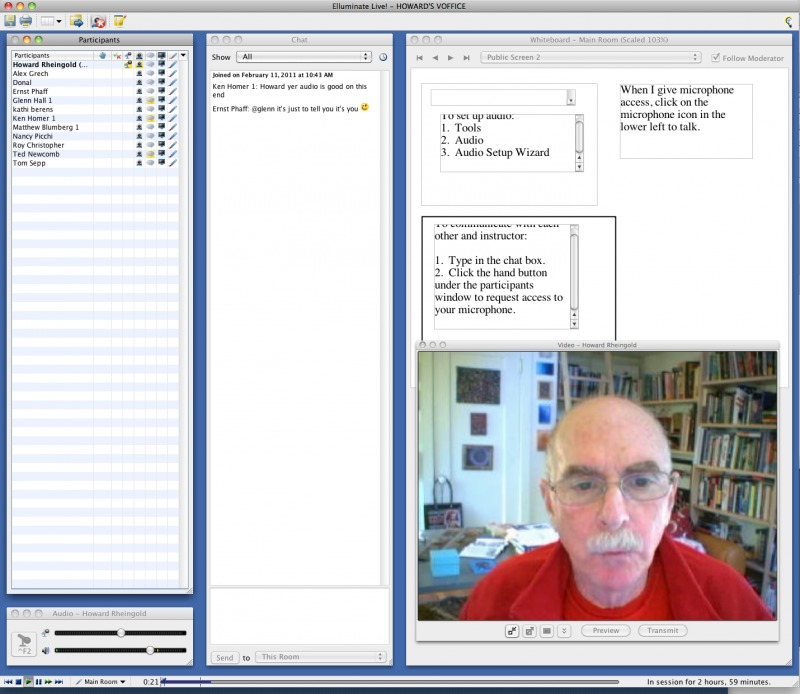
\includegraphics[width=.7\textwidth]{./pictures/elluminate.jpg}
\end{center}

\subsection{Features of real-time meeting platforms}

There are many free services for chat, screen-sharing, whiteboards, and
video conferencing, but combining all these components in separate panes
of the same screen (preferably) or as separate tabs of a browser can
have a powerful synchronizing and harmonizing effect on the group. The
features to look for in meeting platforms include:

\textbf{Audio and video}: Choose platforms that enable
voice-over-internet-protocol (VOIP) and easy ways for participants to
configure their microphones and speakers. Today's webcams, together with
adequate lighting and a broadband connection, enable a number of people
to be visible at the same time. In Blackboard Collaborate, the person
who is speaking at a given moment is visible in the largest video pane,
while other participants are available in smaller video windows. Audio
and video convey much more of a human dimension than text communications
alone. A group of people who have seen and heard each other online are
able to work together via asynchronous media such as forums and wikis
more effectively. Online face-to-face meetings are often the best way
for a group to argue constructively and decide on critical issues.
Forums and email are comparatively bad choices for distributed
decison-making.

\textbf{Slide pushing:} The best platforms will convert .ppt or .pdf
files for sequential display. With the addition of text chat,
annotations to slides, and the ability to ``raise your hand'' or
interrupt with your voice, an online lecture can be a more
multidimensional experience than even a highly discursive in-person
lecture.

\textbf{Text chat:} As a backchannel, a means of quickly exchanging
links to relevant resources, a channel for collaborative note-taking, a
way of communicating with the lecturer and with other participants, text
chat adds a particularly useful dimension to real-time peeragogical
meetings -- especially when the division of labor is explicitly agreed
upon in advance. We've found that even in meetings that use the
real-time collaborative editor \href{http://etherpad.org}{Etherpad} for
collaborative note taking, participants may gravitate toward the
built-in chat box for discussion.

\textbf{Screen sharing:} The ability of participants to show each other
what is on their screens becomes especially important in peer learning,
where we all have some things to show each other.

\textbf{Web tours:} An alternative to screen-sharing is the ability to
display the same web page(s) to all participants by entering URLs.

\textbf{Interactive whiteboards}: A shared space that enables
participants to enter text, drawings, shapes, colors, to move and resize
media, and to import graphic content -- especially if it allows
anonymous actions -- can foster the feeling of participating in a
collective intelligence. Collaborative anonymous mind-mapping of the
discussion is one technique to try with whiteboards. The whiteboard can
also be used to generate an emergent agenda for an ``un-meeting''.

\subsection{Configuring Google+ Hangout - a free alternative for up to
10 people}

For up to 10 people, each equipped with a webcam, microphone, and
broadband connection,
\href{http://lifehacker.com/5842191/google\%252B-hangouts-adds-screen-sharing-google-docs-collaboration-and-more}{Google+
Hangout} can provide high-quality audio-video conferencing. By enabling
the text-chat feature and adding Google Docs, screensharing, and
SketchUp (whiteboard), it is possible to emulate most of what the
commercial services offer. Adobe Connect and Blackboard Collaborate
currently have the user-interface advantage of displaying chat, video,
whiteboard/slides as resizable panes on one screen; at present, the free
Google services can provide a powerful extension of the basic
audio-video platform, but participants have to shift between different
tabs or windows in the browser. Note that it is possible to
\href{http://www.google.com/+/learnmore/hangouts/onair.html}{stream a
Hangout and record it to YouTube}, again at no cost to the user.

\subsection{Suggestions for real-time meetings}

In the nine online courses I have facilitated, the emphasis on
co-learning encouraged participants to suggest and shape active roles
during real-time meetings. By creating and taking on roles, and shifting
from role to role, participants engage in a kind of collective learning
about collective learning which can be as pleasurable as well as useful.
Typically we first brainstorm, then analyze, then organize and present
the knowledge that we discover, construct, and ultimately convey
together.

\subsection{Roles for participants in real-time meetings}

\begin{itemize}
\item
  \textbf{Searchers:}~search the web for references mentioned during the
  session and other resources relevant to the discussion, and publish
  the URLs in the text chat
\item
  \textbf{Contextualizers:} add two or three sentences of contextual
  description for each URL
\item
  \textbf{Summarizers:}~note main points made through text chat.
\item
  \textbf{Lexicographers:}~identify and collaboratively define words and
  phrases on a wiki page.
\item
  \textbf{Mappers:}~keep track of top level and secondary level
  categories and help the group mindmapping exercise at the end of the
  session.
\item
  \textbf{Curators:}~compile the summaries, links to the lexicon and
  mindmaps, contextualized resources, on a single wiki page.
\item
  \textbf{Emergent Agendas:} using the whiteboard for anonymous
  nomination and preference polling for agenda items, with voice, video,
  and text-chat channels for discussing nominations, a group can quickly
  set its own agenda for the real-time session.
\end{itemize}

\subsection{The Paragogical Action Review}

Charlie Danoff and Joe Corneli remixed the US Army's ``After Action
Review'' to make a technique for evaluating peer learning as it happens.
The five steps in the PAR are:

\begin{enumerate}
\item
  Review what was supposed to happen
\item
  Establish what is happening/happened
\item
  Determine what's right and wrong with what we are doing/have done
\item
  What did we learn or change?
\item
  What else should we change going forward?
\end{enumerate}

Participants can run through these steps during live meetings to
reassess the medium, the readings, the group dynamics, or any other
choices that have learning relevance. The focus in the PAR is on change:
as such, it provides a simple way to implement the ``double loop
learning'' of Chris Argris (see references).

\subsubsection{\textbf{References}}

\begin{enumerate}
\item
  Argyris, Chris.
  "\href{http://pds8.egloos.com/pds/200805/20/87/chris\_argyris\_learning.pdf}{Teaching
  smart people how to learn}." Harvard Business Review, 69.3, 1991.
\item
  Charles Jeffrey Danoff, Joseph Corneli, and Dr. Muhammed Bello Umar,
  \href{http://metameso.org/~joe/docs/The-Paragogical-Action-Review.pdf}{The
  Paragogical Action Review}, submitted to \emph{The African Journal of
  Information Systems}.
\end{enumerate}

\subsubsection{\textbf{Resources}}

\begin{itemize}
\item
  Howard Rheingold's webconferencing
  \href{http://delicious.com/hrheingold/webconferencing}{bookmarks}
\item
  \href{http://www.bigbluebutton.org/}{Big Blue Button}
\item
  \href{http://www.blackboard.com/platforms/collaborate/overview.aspx}{Blackboard
  Collaborate}
\item
  \href{http://www.google.com/+/learnmore/hangouts/}{Google Hangouts~}
\item
  \href{http://www.bigmarker.com/about}{Big Marker}
\end{itemize}
